\documentclass[dvipsnames, svgnames, x11names]{beamer}
\usetheme{mytheme}

%封面
\title{第八章}
\subtitle{表面物理化学}
\author{张斌}
\institute[理工系]{河北农业大学 理工系}
\date{\the\year 年 \the\month 月}



\begin{document}

\begin{frame}
	\titlepage
	\thispagestyle{empty}
	\addtocounter{framenumber}{-1}
\end{frame}

    \begin{frame}
        \frametitle{表面物理化学}
    
        表面物理化学(surface physical chemistry)是研究两相之间界面上发生的物理化学过程的科学。两相界面是指相邻两体相间极薄的边界层，厚度可以是单分子层或几个分子层。在本章中，我们将学习：
        \begin{itemize}
            \item 界面现象中的一些基本概念和规律
            
            表面张力、表面自由能、润湿、拉普拉斯公式、开尔文公式、杨氏方程
            \item 液体和溶液的表面特性
            
            表面活性剂、表面膜和胶束
            \item 固体表面特性
            
            弗兰德里希定温式、朗缪尔定温式、BET吸附定温式
        \end{itemize}

    
    \end{frame}

	\begin{frame}{}
        \begin{center}
            {\Huge \cbf{目 \ 录}}
        \end{center}
		\tableofcontents
		\thispagestyle{empty}
		\addtocounter{framenumber}{-1}
	\end{frame}




\section{表面吉布斯自由能}


\begin{frame}
    \frametitle{常见的表面}
    \begin{figure}[htpb]
        \centering
        \setcounter{subfigure}{0}
        \subfloat[气液、液液界面]{
\includegraphics[height=2.5cm]{气液}}\quad
        \subfloat[气固界面]{
\includegraphics[height=2.5cm]{气固}}\\
        \subfloat[液固界面]{
\includegraphics[height=2.4cm]{液固}}\quad
        \subfloat[固固界面]{
\includegraphics[height=2.4cm]{固固}}
    \end{figure}
\end{frame}


\begin{frame}
    \frametitle{界面现象的本质}
    表面层显示出一些独特性质，如表面张力、表面吸附、毛细现象、过饱和状态等。其本质是因为表面层分子与内部分子相比所处的环境不同。

    体相内部分子所受四周邻近相同分子的作用力是对称的，各个方向的力彼此抵销；但是处在界面层的分子，一方面受到体相内相同物质分子的作用，另一方面受到性质不同的另一相中物质分子的作用，其作用力未必能相互抵销，因此，界面层会显示出一些独特的性质。

    \begin{figure}[htpb]
        \centering
        
\includegraphics[width=.5\linewidth]{fig8.1}
    \end{figure}
\end{frame}


\begin{frame}
    \frametitle{比表面}

    表面现象显著的体系常是高度分散的体系，如粉末状或多孔状物质、水中的气泡、油滴等。衡量多相分散体系的分散程度通常用比表面(specific surface)表示
    \[
        S_0 = \frac{A}{V} \quad \text{或} \quad S_0 = \frac{A}{m}
    \]
    式中$A$为体积为$V$或质量为$m$的物质所具有的总表面积。
    
    比表面$S_0$就是单位体积或单位质量的物质所具有的表面积，单位是$m^{-1}$或\si{m^2.kg^{-1}}。
    
    当将固体颗粒或液滴的尺寸逐渐降低时，比表面$S_0$的数值将随之迅速增加。

\end{frame}


\begin{frame}[t]{}
    \begin{example}
        一滴体积$V = \SI{e-6}{m^3}$的水滴，当被分散为半径分别是$r_1 = \SI{e-3}{m}$，$r_2 = \SI{e-4}{m}$，$r_3 = \SI{e-6}{m}$和$r_4 = \SI{e-8}{m}$的小液滴时，分散成的水滴总数、比表面和总表面积各为多少？
    \end{example}\pause
    \begin{table}[]
        \begin{tabular}{cccc}
        \hline
        水滴半径/m & 液滴数目 & 比表面$S_0/\mathrm{m}^{-1}$ & 总表面积$A/\mathrm{m}^{2}$ \\ \hline
        $6.2\times 10^{-3}$ & 1 & $4.8\times 10^2$ & $4.8\times 10^{-4}$ \\
        $10^{-3}$ & $2.4\times 10^2$ & $3\times 10^3$ & $3\times 10^{-3}$ \\
        $10^{-4}$ & $2.4\times 10^5$ & $3\times 10^4$ & $3\times 10^{-2}$ \\
        $10^{-6}$ & $2.4\times 10^{11}$ & $3\times 10^6$ & 3 \\
        $10^{-8}$ & $2.4\times 10^{17}$ & $3\times 10^8$ & $3\times 10^2$ \\ \hline
        \end{tabular}
        \end{table}

\end{frame}


\begin{frame}
    \frametitle{比表面自由能}

        \begin{minipage}{0.48\linewidth}
            表面层分子与体相内分子所处环境不同。表面层分子主要受到指向液体内部的拉力，使得表层分子有向液体内部迁移、液体表面积自动收缩的趋势。
        \end{minipage}\hfill
        \begin{minipage}{0.48\linewidth}
            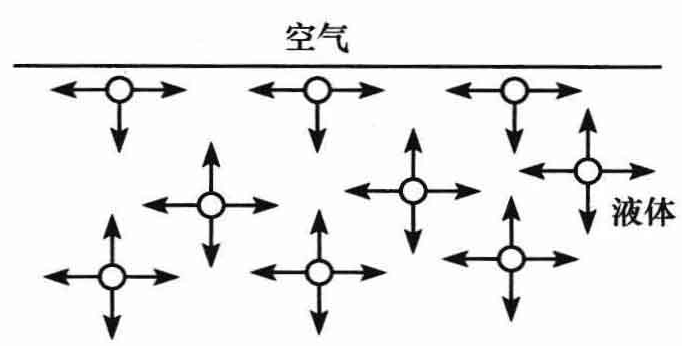
\includegraphics[width=\linewidth]{figures/fig8.1.png}
        \end{minipage}

        \highlight{表面功}：如果要扩大液体表面，即把一些分子从液相内部移到表面上，就必须克服液体内部分子之间的吸引力而对体系做功，此功称为表面功。

        定温、定压，组成恒定时，
        \[
            \delta W' = \sigma\dif A
        \]
        表面功$\delta W'$为可逆非体积功，$\sigma$为比例常数。
\end{frame}


\begin{frame}
    \frametitle{比表面自由能}

    定温定压下体系可逆地扩展表面所得到的表面功应等于吉布斯自由能的增加量，$\dif G = \delta W'$。
    \[
        \dif G = \sigma\dif A \qquad \text{或} \qquad \sigma = \left(\frac{\partial G}{\partial A}\right)_{T,p,n}
    \]
    $\sigma$的物理意义是当$T$、$p$及组成恒定时，增加单位表面积所引起的吉布斯自由能的增量。
    
    $\sigma$称为比表面自由能，单位\si{J.m^{-2}}。
    
    当可逆地形成新表面时，环境所做的表面功转化为表面层分子的吉布斯自由能。表层分子因此比体相内分子具有更高的能量，$\sigma$也称为表面过剩吉布斯自由能，简称表面能。

\end{frame}


\begin{frame}
    \frametitle{表面张力}

    表面现象还可以从力的角度描述。气-液界面两边物质不同，其密度也不同，故液体表面存在使其面积减小的力，称为表面张力（或界面张力）。其物理意义是在与液面相切方向上垂直作用于单位长度线段上的收缩力。表面张力也用符号$\sigma$表示，单位为\si{N.m^{-1}}。表面张力与比表面自由能在数值上完全相等，并有相同的量纲，但物理意义不同，是从不同角度反映体系的表面特征。

    表面张力的大小与物质种类、共存另一相的性质以及温度和压力等因素有关。
    
    测量表面张力的方法有：
    \begin{enumerate}
      \item 吊板法
      \item 滴重法
      \item 最大泡压法
      \item 毛细管上升法
    \end{enumerate}

\end{frame}
\section{弯曲液面的特性}


\begin{frame}
    \frametitle{弯曲液面的附加压力}

    表面弯曲的液体与平面液体有所不同，因为表面张力的存在，总是力图收缩液体表面积，这导致弯曲液体界面上承受着一定的附加压力。
    \begin{figure}[htpb]
        \centering
        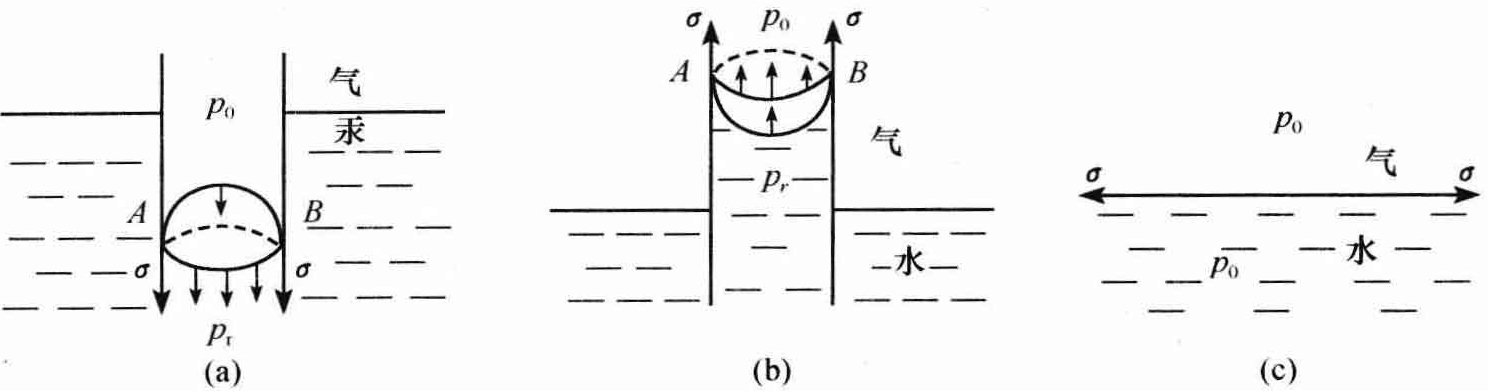
\includegraphics[width=\linewidth]{figures/fig8.2.png}
    \end{figure}
    \begin{itemize}
        \item 凸面，表面张力方向与周界垂直，指向汞的内部。 $\Delta p = p_r - p_0 > 0$
        \item 凹面，在交界线AB上作用的表面张力方向指向气相。$\Delta p < 0$
    \end{itemize}

\end{frame}


\begin{frame}
    \frametitle{拉普拉斯公式}

        \begin{minipage}{0.78\linewidth}
            若给毛细管上方活塞稍稍加压，可逆地使液滴半径增大d$r$，
            \[
                \delta W' = \dif G
            \]
            \[
                \Delta p \dif V = \sigma \dif A
            \]
            \[
                \Delta p \times 4 \pi r^2 \dif r = \sigma \times 8 \pi r \dif r
            \]
            \[
                \magenta{\Delta p = \frac{2\sigma}{r}}
            \]            
        \end{minipage}\hfill
        \begin{minipage}{0.18\linewidth}
            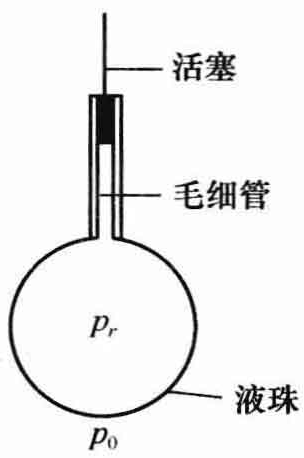
\includegraphics[width=\linewidth]{figures/fig8.3.png}
        \end{minipage}

        \begin{itemize}
            \item 附加压力与曲率半径有关。液滴越小，则所受到的附加压力值$\Delta p$越大。
            \item 弯曲液面为凸面，曲率半径为正，$r>0$，$\Delta p >0$。凹面反之。
            \item 空气中的肥皂泡，泡内气体压力大于泡外压力，因液膜有内外两个表面，其半径也近似相同，压力差值$\Delta p = \frac{4\sigma}{r}$。
            \item 平面液体，曲率半径$r \to \infty$，$\Delta p =0$。
        \end{itemize}

\end{frame}


\begin{frame}[t]
    \frametitle{}
    \begin{example}
        玻璃管两端各有一大一小肥皂泡，若将中间的旋塞打开使两气泡相通，将发生什么变化？为什么？
        \begin{figure}[htpb]
            \centering
            
\includegraphics[width=.4\linewidth]{肥皂泡}
        \end{figure}
    \end{example}
\end{frame}


\begin{frame}
    \frametitle{拉普拉斯公式的应用$-$毛细管法测液体表面张力}

    当把毛细管插入水中时，管中水柱呈凹形曲面，并上升至一定高度$h$。
    \[
        \Delta p = \frac{2\sigma}{r} = \Delta \rho gh
    \]
    $\Delta \rho = \rho_\text{液} - \rho_\text{气}$，一般$\rho_\text{液} \gg \rho_\text{气}$，故
    \[
        h = \frac{2\sigma}{\rho gr} = \frac{2\sigma}{\rho gR}
    \]
        \begin{minipage}{0.78\linewidth}
            因水能润湿玻璃毛细管，故弯曲面的曲率半径$r$近似于毛细管半径$R$。测定了毛细上升高度$h$和管径$R$，可求出液体的表面张力值。

            更一般的情况是管内液面只是球面的一部分，$R = r \cos \theta$
            \[
                h = \frac{2\sigma \cos \theta}{\rho gR}
            \]
        \end{minipage}\hfill
        \begin{minipage}{0.18\linewidth}
            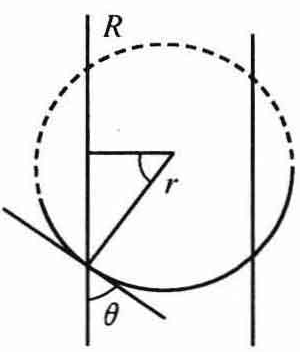
\includegraphics[width=\linewidth]{figures/fig8.5.png}
        \end{minipage}
    
\end{frame}


\begin{frame}
    \frametitle{弯曲液面的蒸气压}

    设在一定温度时，1 mol平面液体与其蒸气达到平衡，$\mu _\mathrm{l} = \mu _\mathrm{g}$。若液面曲率发生变化，如将平面液体分散成半径为$r$的小液滴，因附加压力的存在，液体所受压力由$p_0$变成$p_r$，相应地其饱和蒸气压发生改变，由$p_0^*$变为$p_r^*$，并重新建立平衡，$\dif \mu _\mathrm{l} = \dif \mu _\mathrm{g}$。当温度一定时，对于纯液体$\dif \mu _\mathrm{l} = V_\mathrm{m,l} \dif p$。假定蒸汽为理想气体，$\dif \mu _\mathrm{g} = V_\mathrm{m,g} \dif p^* = \frac{RT}{p^*}\dif p^* = RT \dif \ln p^*$，故
    \[
        V_\mathrm{m,l} \dif p = RT \dif \ln p^* 
    \]
    积分
    \[
        \int_{p_{0}}^{p_{r}} V_{\mathrm{m}, 1} \mathrm{~d} p=\int_{p_{0}^{*}}^{p_{r}^{*}} R T \mathrm{~d} \ln p^{*}
    \]
    \[
        V_{\mathrm{m}, l}(p_{r}-p_{0})=R T \ln \frac{p_{r}^{*}}{p_{0}^{*}}
    \]

\end{frame}


\begin{frame}
    \frametitle{弯曲液面的蒸气压}

    $p_{r} - p_{0} = \frac{2\sigma}{r}$，液体的摩尔体积$V_\mathrm{m,l} = \frac{M}{\rho}$，于是
    \[
        \magenta{\ln \frac{p_{r}^{*}}{p_{0}^{*}}=\frac{2 \sigma M}{\rho R T} \frac{1}{r} \qquad \text{(开尔文公式)}}
    \]
    液珠的蒸气压大于平面液体的蒸气压，且液珠半径越小，蒸气压越大。

    凸面液体的饱和蒸气压比平面的高，而凹液面的蒸气压比平面液体的要低。
    \begin{table}[ht]
    \caption{298K时水滴半径与蒸汽压的关系}
    \begin{tabular}{@{}ccccc@{}}
    \toprule
    $r/\mathrm{m}$ & $10^{-6}$ & $10^{-7}$ & $10^{-8}$ & $10^{-9}$  \\ \midrule
    $p_{r}^{*}/p_{0}^{*}$ & 1.001 & 1.011 & 1.111 & 2.859 \\ \bottomrule
    \end{tabular}
    \end{table}
    水蒸气在相对纯净的高空中可以达到很高的过饱和程度而不凝聚成水滴。

\end{frame}


\begin{frame}[t]
    \frametitle{}
    \begin{example}
        在一个封闭的钟罩内，有大小不等的两个球形液滴，问长时间恒温放置后会出现什么现象。
    \end{example}
\end{frame}

% 如果液体上方的蒸气压小于饱和蒸气压，那么液体就会挥发，直到蒸气压等于饱和蒸气压为止。所以如果饱和蒸汽压越大，液体就越容易蒸发，以达到液－气平衡。
\section{溶液的表面吸附}


\begin{frame}
    \frametitle{溶液的表面张力}

    在一定温度、压力下，纯液体的表面张力是一定值。溶液的表面张力不仅与温度、压力有关，还与溶质的种类及浓度有关。

    在水溶液中，表面张力随组成的变化有三种类型：
        \begin{minipage}{0.58\linewidth}            
            \begin{itemize}
                \item[I] 无机盐、非挥发性的酸或碱以及蔗糖、甘露醇等多羟基有机物\magenta{(表面惰性物质)}
                \item[II] 短链醇、醛、酮、酸和胺等有机物
                \item[III] 碳原子数为8个以上的直长链有机酸碱金属盐、磺酸盐、硫酸盐和苯磺酸盐等
                
                \magenta{(表面活性物质，表面活性剂)}
            \end{itemize}
        \end{minipage}\hfill
        \begin{minipage}{0.38\linewidth}
            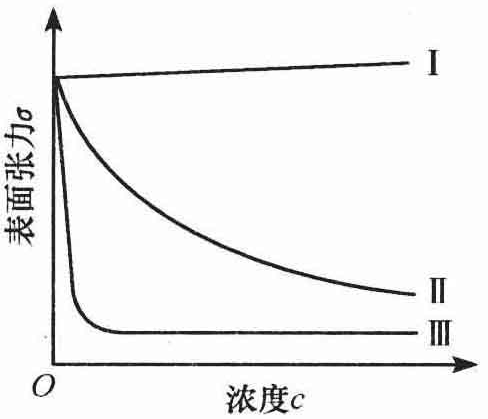
\includegraphics[width=\linewidth]{figures/fig8.6.png}
        \end{minipage}

\end{frame}


\begin{frame}
    \frametitle{吉布斯吸附定温式}

    溶液表面层与体相溶液组成不同的现象称为溶液表面吸附。
    \begin{itemize}
      \item 溶质在表面相浓度高于液相内部，使溶液的表面张力降低
      \item 溶质在表面相浓度低于其在液相内部的浓度，使溶液的表面张力升高
    \end{itemize}

    吉布斯用热力学方法导出了一定温度下，联系溶液的表面张力、溶液浓度和吸附量的微分方程，通常称为吉布斯吸附定温式。
    \[
        \varGamma =-\frac{c}{R T}\left(\frac{\partial \sigma}{\partial c}\right)_{T}
    \]
    $\varGamma$为单位面积表面相中吸附溶质的过剩量，又称表面过剩量。
    
    \begin{itemize}
        \item 若$\left(\frac{\partial \sigma}{\partial c}\right)_{T}<0$， 则$\varGamma > 0$。表面张力随着溶质的加入而降低者，是正吸附。
        \item 若$\left(\frac{\partial \sigma}{\partial c}\right)_{T}>0$， 则$\varGamma < 0$。表面张力随着溶质的加入而升高者，是负吸附。
    \end{itemize}
\end{frame}


\begin{frame}
    \frametitle{吸附量与浓度的关系}

    一定温度下实验测定不同浓度$c$对应的溶液表面张力值$\sigma$。以$\sigma$对$c$作图，在$\sigma - c$曲线上作切线，指定浓度下切线的斜率即为该浓度的$\left(\frac{\partial \sigma}{\partial c}\right)_{T}$值，再由吉布斯吸附定温式，即可得浓度时的表面吸附量$\varGamma$。作$\varGamma - c$曲线，称为吸附定温线。

        \begin{minipage}{0.61\linewidth}
            \begin{itemize}
                \item 溶质浓度很小时，$\varGamma$与$c$的关系近似直线，吸附量随溶质浓度的增加而增大；
                \item 当浓度足够大时，表面吸附量趋近一极限值$\varGamma_\mathrm{m}$，此时溶液表面的吸附已达饱和。
                \item 再增加浓度，表面吸附量不再改变，$\varGamma_\mathrm{m}$为一定值，与浓度无关。$\varGamma_\mathrm{m}$称为饱和吸附量。
            \end{itemize}
        \end{minipage}\hfill
        \begin{minipage}{0.37\linewidth}
            \begin{figure}[htpb]
                \centering                
                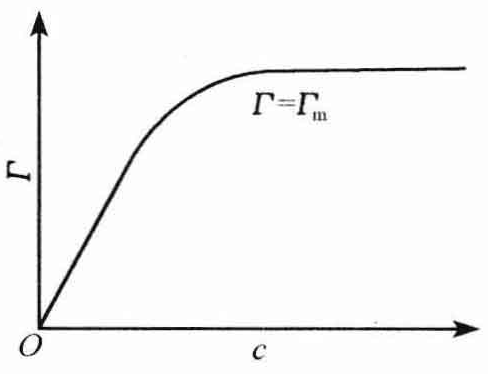
\includegraphics[width=.9\linewidth]{figures/fig8.7.png} 
                \caption{表面活性物质的吸附定温线}
            \end{figure}
        \end{minipage}

\end{frame}


\begin{frame}
    \frametitle{吸附层上分子的定向排列}

    表面活性物质分子具有两亲特性，分子的一端是亲油的非极性基团，另一端是极性基团，其亲水作用使分子的极性端进入水中。当浓度较高，溶质分子在表面层达饱和吸附时，分子在表面定向排列成单分子膜。
    \begin{figure}[htpb]
        \centering
        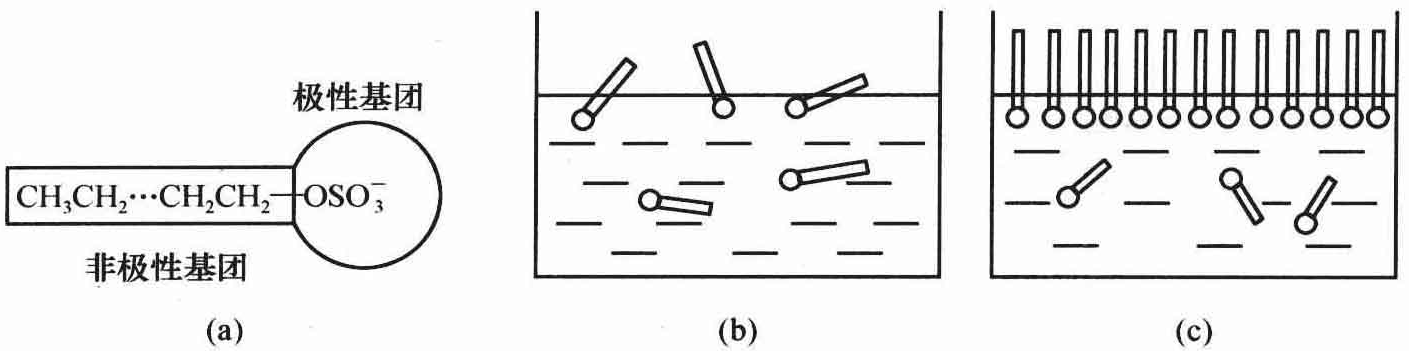
\includegraphics[width=\linewidth]{figures/fig8.8.png}
    \end{figure}
    \[
       \text{分子截面积} \quad A = \frac{1}{L \varGamma_\mathrm{m}}
    \]

\end{frame}

\section{表面活性物质}


\begin{frame}
    \frametitle{表面活性物质的分类}

\begin{table}[]
    \begin{tabular}{cc|l}
    \Xhline{1pt}
    \rowcolor{maincolor!10}
    \multicolumn{2}{c|}{类别} & \multicolumn{1}{c}{实例} \\ \hline
    \multicolumn{1}{l|}{\multirow{6}{*}{\makecell{离子\\型\\表面\\活性\\物质}}}  &  \multirow{2}{*}{阴离子型} & 羧酸盐\ch{RCOO^-M+}，硫酸酯盐\ch{ROSO3^-M+}   \\ 
    \multicolumn{1}{l|}{}  &   &  磺酸盐\ch{RSO3^-M+}，磷酸酯盐\ch{ROPO3^-M+}                \\ \cline{2-3} 
    \multicolumn{1}{l|}{}  &  \multirow{2}{*}{阳离子型} &  伯胺盐\ch{RNH3^+X^-}，季胺盐\ch{RN^+(CH3)3X^-}\\ 
    \multicolumn{1}{l|}{}  &   &  吡啶盐                \\ \cline{2-3} 
    \multicolumn{1}{l|}{}  &  \multirow{2}{*}{两性离子型} &  氨基酸型\ch{RN^+CH2CH2COO^-}              \\ 
    \multicolumn{1}{l|}{}  &   &  甜菜碱型\ch{RN^+(CH3)2CH2COO^-}                 \\ \hline
    \multicolumn{2}{c|}{\multirow{3}{*}{非离子型表面活性物质}}  &   聚氧乙烯醚\ch{RO(CH2CH2O)_n H}   \\ \cline{3-3} 
    &   &  聚氧乙烯酯\ch{RCOO(CH2CH2O)_nH}    \\ \cline{3-3} 
    &   &  多元醇型\ch{RCOOCH2C(CH2OH)3}      \\ \Xhline{1pt}
    \end{tabular}
    \end{table}

\end{frame}


\begin{frame}
    \frametitle{表面活性物质的HLB值}

    格里芬(Griffin)提出用HLB(hydrophile-lipophile balance)，即亲水$-$亲油平衡值来表示表面活性物质的亲水性和亲油性的相对强弱。
    \begin{itemize}
      \item HLB越大，其亲水性越强；
      \item HLB越小，其亲水性越弱，亲油性越强。
      \item 表面活性物质的HLB是个相对值。
    \end{itemize}
    \begin{table}[]
      \caption{HLB范围及其适当用途}
      \begin{tabular}{cc|cc}
        \Xhline{1pt}
      \rowcolor{maincolor!10}
      HLB & 应用           & HLB   & 应用           \\ \hline
      1-3 & 消泡剂          & 8-18  & O/W(水包油)型乳化剂 \\
      3-6 & W/O(油包水)型乳化剂 & 13-15 & 洗涤剂          \\
      7-9 & 润湿剂          & 15-18 & 增溶剂          \\ \Xhline{1pt}
      \end{tabular}
      \end{table}
\end{frame}
\section{胶束}


\begin{frame}
    \frametitle{表面活性物质的临界胶束浓度}

    当表面活性物质浓度增至一定值，在表面层上，物质吸附达饱和，表面活性物质分子形成单分子层。表面层容纳不下的表面活性物质分子在溶液中以疏水基相互靠拢，形成以疏水基朝内、亲水基指向水相的胶束。形成胶束的浓度称为表面活性物质的临界胶束浓度，简称CMC，影响CMC的因素主要是分子的结构。
    \begin{figure}[htpb]
        \centering
        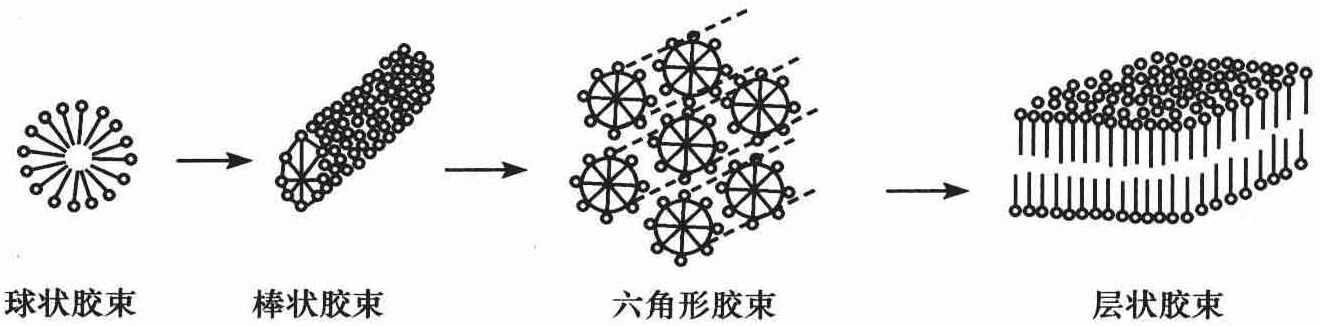
\includegraphics[width=.7\linewidth]{figures/fig8.12.png}
    \end{figure}
    \begin{itemize}
        \item 胶束的形状与形成胶束的浓度有关
        \item 胶束的大小与构成胶束的表面活性物质分子的数目即聚集数有关
    \end{itemize}

\end{frame}


\begin{frame}
    \frametitle{增溶作用}

    表面活性物质水溶液的一个重要应用，是能溶解一些原来不溶或微溶于水的物质。增溶作用的特征如下：
    \begin{enumerate}
        \item 增溶作用必须在CMC以上的浓度才能发生，即胶束的存在是发生增溶作用的必要条件，而且浓度越大，胶束越多，增溶效果越显著。
        \item 增溶作用是一热力学自发过程，可使被增溶物的蒸气压下降，化学势降低，增溶后体系更为稳定。
        \item 增溶后溶液为透明的体系，而且溶剂的依数性质基本不变。说明增溶并非溶解，溶质在增溶过程中并未在溶剂中分散成分子或离子状态，而是溶入胶束。溶液中质点总数未增加，只是胶束胀大。
        \item 增溶作用是一可逆的平衡过程。无论用什么方法，达到平衡后的增溶结果是一样的。
    \end{enumerate}

\end{frame}
\section{气-固界面吸附}


\begin{frame}
    \frametitle{固体表面特性}

    \begin{enumerate}
        \item 固体表面不均匀
        
        绝大多数固体表面是不规则的，即使磨光的表面也会有$10^{-5} \sim 10^{-3}$cm的不规则性，也就是说表面总是粗糙不平的。
        \item 固体表面分子、原子或离子较难移动
        
        固体表面上的原子、分子或离子的力场是不均衡的，固体表面也有表面张力和表面能。固体具有固定的形状，其表面分子、原子或离子通常难移动。
        \item 固体表面层的组成与体相组成不同
        
        固体表面的各种性质不是内部性质的延续，表面处理方式不同或固体形成条件不同，固体表面层由表向里往往呈现出多层次结构。
    \end{enumerate}

\end{frame}


\begin{frame}
    \frametitle{吸附和吸附平衡}

    固体暴露在气体中时，气体分子自动聚集在固体表面上，这种现象称为吸附。
    \begin{itemize}
        \item 吸附剂：具有吸附作用的物质
        \item 吸附质：被吸附的物质
    \end{itemize}

    在气-固吸附体系中，同时存在着两个相反的过程：
    \begin{itemize}
        \item 吸附：气体分子在表面力场的作用下，在吸附剂表面聚集
        \item 脱附：已吸附在固体表面上的气体分子会逃离吸附剂表面
    \end{itemize}
    吸附和解吸是互逆的两个过程，当这两个过程速率相等时，达到吸附平衡。吸附平衡是动态平衡。

\end{frame}


\begin{frame}
    \frametitle{吸附量和吸附热}

    吸附剂吸附气体的能力可用吸附量来表示
    \[
        \varGamma(\text{吸附量}) = \frac{n(\text{气体的物质的量})}{m(\text{吸附剂的质量})} \qquad (\si{mol.kg^{-1}})
    \]
    \[
        \varGamma(\text{吸附量}) = \frac{V(\text{273K，标准状态下气体的体积})}{m(\text{吸附剂的质量})} \qquad (\si{m^3.kg^{-1}})
    \]
    吸附是自发的，吸附过程中吉布斯自由能减少$\Delta G < 0$。

    当气体分子在固体表面上吸附后，气体分子从原来空间的三维运动变成限制在表面层上的二维运动，运动自由度减少，因而熵也减少$\Delta S < 0$。
    
    定温下$\Delta H = \Delta G - T \Delta S < 0$，所以吸附通常都是放热过程。
    
    吸附过程中产生的热量称为吸附热，吸附热的大小可以衡量吸附的强弱程度，吸附热越大，吸附越强。

\end{frame}


\begin{frame}
    \frametitle{物理吸附和化学吸附}

    气体在固体表面上的吸附，可分为物理吸附和化学吸附两种类型。
    \begin{table}        
            \caption{物理吸附与化学吸附的比较}
            \begin{tabular}{ccc}
                \Xhline{1pt}
                \rowcolor{maincolor!10}
                吸附性质 & 物理吸附 & 化学吸附\\
                \hline
                吸附力 & 分子间引力 & 化学键力\\
                选择性 & 无，所有气体都可被吸附 & 有，不是所有气体都可被吸附\\
                吸附温度 & 低温，温度升高吸附量减小 & 高温，温度升高吸附速率增加\\
                吸附热 & 较小，$8\sim 25\si{kJ.mol^{-1}}$ & 较大，$40\sim 200\si{kJ.mol^{-1}}$\\
                吸附层数 & 多层吸附 &单层吸附 \\
                稳定性 & 不稳定，已解吸 & 比较稳定 \\
                应用 & 测定固体表面积及孔径大小 & 测定表面浓度，吸附和解吸速率\\
                \Xhline{1pt}
            \end{tabular}        
    \end{table}

\end{frame}


\begin{frame}
    \frametitle{吸附定温线和吸附定温式}

    实验表明，气体在固体表面上的吸附量$\varGamma$与气体的性质、固体的性质、表面状态、表面大小，以及吸附平衡时温度$T$、气体的压力$p$等有关，可表示为：
    \[
        \varGamma = f(T,p)
    \]
    \vspace{-20pt}
    \begin{itemize}
        \item 若$T=$常数，则$\varGamma = f(p)$，称为吸附定温式
        \item 若$p=$常数，则$\varGamma = f(T)$，称为吸附定压式
        \item 若$\varGamma=$常数，则$p = f(T)$，称为吸附定量式
    \end{itemize}
    若用平面上的曲线表示上述三个式子，则分别得到吸附定温线、吸附定压线和吸附定量线。这三组曲线互相关联，其中最常用的是吸附定温线。吸附定温线可由实验测出。

\end{frame}


\begin{frame}
    \frametitle{吸附定温线和吸附定温式}

    由于气体与固体分子间作用力的不同，以及固体表面状态的差异，吸附定温线的形状是多种多样的。
    \begin{figure}[htpb]
        \centering
        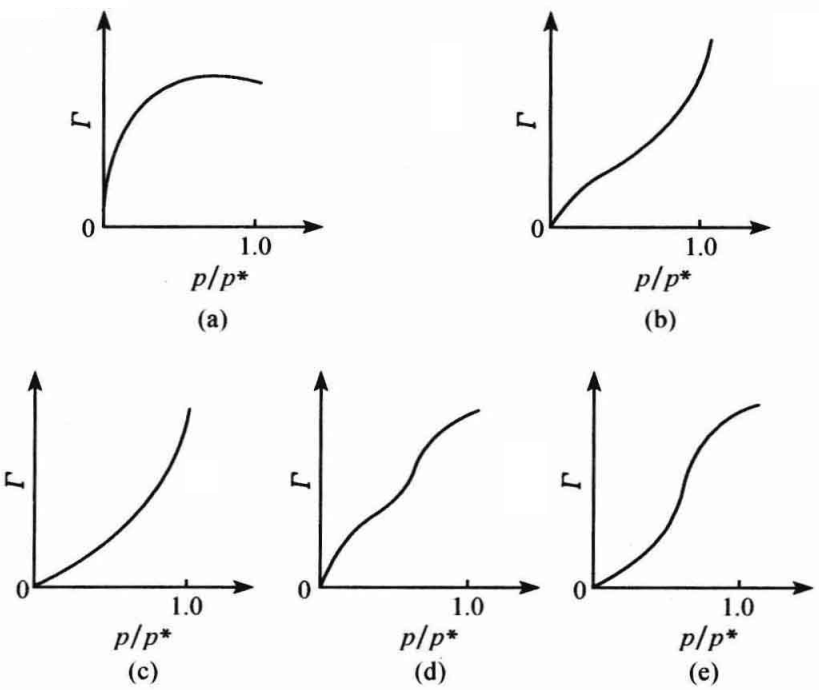
\includegraphics[width=.45\linewidth]{figures/fig8.15.png}
    \end{figure}

\end{frame}


\begin{frame}
    \frametitle{吸附理论}

    \begin{itemize}
        \item[1.] \cbf{弗兰德里希定温式}
    \end{itemize}
    根据实验结果，弗兰德里希（Freundlich）提出一个经验公式
    \[
        \varGamma = kp^{1/n} \qquad (n>1)
    \]
    取对数
    \[
        \lg \varGamma = \frac{1}{n} \lg p + \lg k
    \]
    以$\lg \varGamma$对$\lg p$作图得一直线，截距为$\lg k$，斜率为$\frac{1}{n}$。可求得k和n的值。

    弗兰德里希定温式在中等压力范围内能较好地适用于(a)类定温线，有一定的用途，但是它只是一个经验式，没有提供任何关于吸附机理的信息，只能代表一部分事实。

\end{frame}


\begin{frame}
    \frametitle{吸附理论}

    \begin{itemize}
        \item[2.] \cbf{朗缪尔定温式及单分子层吸附理论}
    \end{itemize}

    朗缪尔单分子层吸附理论的基本假设如下：
    \begin{enumerate}
        \item 催化剂表面各处的吸附能力是均匀的，各吸附位具有相同的能量        
        \item 吸附是单分子层的
        \item 被吸附分子间不发生相互作用，吸附分子的解吸概率不受邻近其他吸附分子的影响
        \item 吸附是一个可逆过程，气体在固体表面上的吸附是气体分子的吸附与解吸两种相反过程达到动态平衡的结果。
    \end{enumerate}
    定温下吸附平衡时，吸附速率等于解吸速率
    \[
        k_1p(1-\theta) = k_{-1}\theta
    \]

\end{frame}


\begin{frame}
    \frametitle{吸附理论}

    \begin{itemize}
        \item[2.] \cbf{朗缪尔定温式及单分子层吸附理论}
    \end{itemize}
    \[
        \theta=\frac{k_{1} p}{k_{-1}+k_{1} p} = \frac{\varGamma}{\varGamma_{\mathrm{m}}}
    \]
    令$b = \frac{k_1}{k_{-1}}$，则
    \[
        \varGamma=\varGamma_{\mathrm{m}} \theta=\varGamma_{\mathrm{m}} \frac{b p}{1+b p}
    \]
    \[
        \frac{p}{\varGamma}=\frac{1}{\varGamma_{\mathrm{m}} b}+\frac{p}{\varGamma_{\mathrm{m}}}
    \]
    上述式子均称为朗缪尔吸附定温式。$b$是吸附平衡常数，其大小代表了固体表面吸附气体能力的强弱。$\varGamma_{\mathrm{m}}$和$b$在一定温度下对一定吸附体系是常数。

    朗缪尔吸附定温式能很好地符合图(a)，可以较好地说明化学吸附。但是由于该理论假设固体表面均匀且只能形成单分子层，因此在实用中有一定的局限性。

\end{frame}


\begin{frame}
    \frametitle{吸附理论}

    \begin{itemize}
        \item[3.] \cbf{BET吸附定温式及多分子层吸附理论}
    \end{itemize}
    由于大多数固体对气体的吸附并不是单分子层吸附，尤其是物理吸附，往往是多分子层吸附，因此其吸附定温线不符合朗缪尔定温式。1938年，Brunauer、Emmett、Teller在朗缪尔理论的基础上，提出了多分子层吸附理论，并推导出著名的BET公式。

    多分子层吸附理论的其改进之处是假设：
    \begin{enumerate}
        \item 吸附是多分子层的
        \item 第一层是气体分子与固体表面分子直接作用引起的吸附，而第二层以后则是气体分子间相互作用产生的吸附。
        \item 在一定温度下，当吸附达到平衡时，气体的吸附量$\varGamma$等于各层吸附量的总和。
    \end{enumerate}

\end{frame}


\begin{frame}
    \frametitle{吸附理论}

    \begin{itemize}
        \item[3.] \cbf{BET吸附定温式及名分子层吸附理论}
    \end{itemize}
    经过比较复杂的数学运算，BET推出定温下吸附平衡时
    \[
        \varGamma=\frac{\varGamma_{\mathrm{m}} C p}{(p^{*}-p)\left[1+(C-1) \frac{p}{p^{*}}\right]}
    \]
    \begin{itemize}
        \item $\varGamma$为平衡压力$p$时的吸附量；
        \item $\varGamma_{\mathrm{m}}$为固体表面盖满单分子层时的吸附量；
        \item $p^*$为实验温度下气体的饱和蒸气压；
        \item $C$为与吸附热有关的常数，反映固体表面和气体分子间作用力的强弱程度
        \item BET吸附定温式也有一定的局限性，不能说明所有的吸附定温线。
    \end{itemize}

\end{frame}


\begin{frame}
    \frametitle{吸附与催化}

    吸附与催化是密切相关的。
    
    发现气-固相的多相催化作用是通过反应分子在催化剂表面上的吸附来实现的。反应分子首先吸附在固体表面的某些部位上，形成活化的表面中间化合物，使反应的活化能降低，反应加速，再经过脱附而得到产物。
        \begin{minipage}{0.68\linewidth}
            对于气-固相催化反应来说，固体表面是反应的场所，比表面的大小直接影响反应速率。因此多采用比表面大的海绵状或多孔性的催化剂。

            固体表面是不均匀的，在表面上有活性的地方只占催化剂表面的很少部分，只有当反应物被吸附到活性中心上才能形成化学键。

            催化剂的催化活性与化学吸附的强弱有密切的关系。
        \end{minipage}\hfill
        \begin{minipage}{0.28\linewidth}
            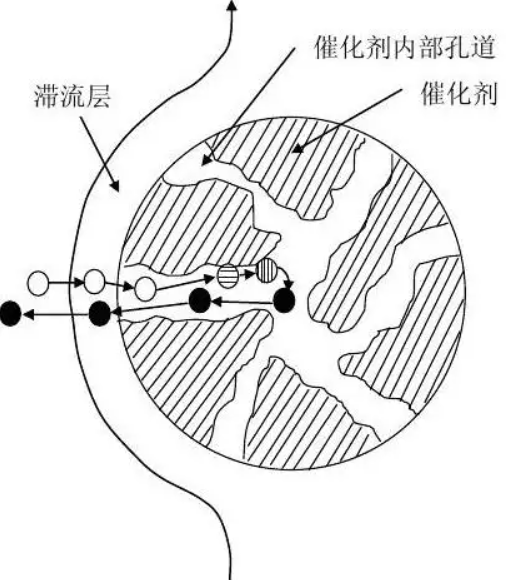
\includegraphics[width=\linewidth]{figures/catalyst.png}
        \end{minipage}
    

\end{frame}
\section{液-固界面吸附}


\begin{frame}
    \frametitle{溶液中吸附量的测定}

    固体在溶液中的吸附较为复杂，因为吸附剂既要吸附溶质，又要吸附溶剂，溶质和溶剂之间还有相互作用。
    
    溶液中的吸附虽然很复杂，但吸附量的测定却比较简单。通常是在定温条件下，将一定量的固体吸附剂与一定量已知浓度的溶液混合，达到吸附平衡后分析溶液的成分。从吸附前后溶液浓度的改变可求出固体对溶质的吸附量。
    \[
        \varGamma = \frac{x}{m} = \frac{V(c_1 - c_2)}{m}
    \]
    式中：$m$为吸附剂的质量；$c_1$和$c_2$分别为溶液起始和平衡的浓度；$V$为溶液的体积，$x$为被$m$g吸附剂所吸附溶质的物质的量。$\varGamma$实际上是固体吸附溶质、溶剂的总结果，称为表观或相对吸附量。 
    
    如果溶液很稀，固体吸附溶剂所造成的浓度变化可以忽略，求得的吸附量可近似看作溶质的吸附量。

\end{frame}


\begin{frame}
    \frametitle{稀溶液中溶质分子的吸附}

    \begin{itemize}
        \item[1.] \cbf{吸附定温线}
    \end{itemize}
    对于不同的体系，吸附定温线的形状不同，有些液-固体系可以使用某些气-固吸附的定温式。
    
    用弗兰德里希定温式表示稀溶液中吸附量与平衡浓度的关系
    \[
        \varGamma = \frac{x}{m} = kc^{\frac{1}{n}}
    \]
    有些稀溶液体系可以用朗缪尔方程来描述其吸附定温线
    \[
        \varGamma = \frac{x}{m} = \frac{\varGamma_\mathrm{m} bc}{1 + bc}
    \]
    如果测出$\varGamma_\mathrm{m}$值和溶质分子截面积$a$，则可以估算出吸附剂的比表积$S_0$
    \[
        S_0 = \varGamma_\mathrm{m} La
    \]

\end{frame}


\begin{frame}
    \frametitle{稀溶液中溶质分子的吸附}
    \begin{itemize}
        \item[2.] \cbf{影响吸附的因素}
    \end{itemize}
    由于溶液中的各组分都能被固体表面吸附，组分之间又存在着相互作用，因此影响吸附的因素较复杂。在长期的实践中，总结出了一些经验规律：
    \begin{itemize}
        \item \bf{极性的影响}
        
        一般说来，极性吸附剂在非极性溶剂中优先吸附极性强的溶质，而非极性的吸附剂在极性溶剂中优先吸附非极性强的溶质。
        \item \bf{溶质溶解度的影响}
        
        溶质溶解度越小，说明溶质与溶剂之间的相互作用越弱，溶质越容易从溶液中析出，较易被吸附。
        \item \bf{温度的影响}
        
        一般情况下，温度升高，吸附量下降。
    \end{itemize}

\end{frame}


\begin{frame}
    \frametitle{电解质溶液中离子的吸附}

    固体在电解质溶液中对离子的吸附通常有两种：
    \begin{itemize}
        \item \bf{离子选择性吸附}
        
        固体在电解质溶液中，可以优先地吸附某种电荷的离子（正离子或负离子），而使固体带有电荷（正或负），这种现象称为离子的选择性吸附。
        \item \bf{离子交换吸附}
        
        离子交换吸附不是固体直接从溶液中吸附离子，而是固体吸附剂本身的组成离子与溶液中的同号离子发生交换，即固体吸附剂在溶液中吸附了某种离子的同时，将另一种相同符号电荷的离子释放到溶液中。
    \end{itemize}

\end{frame}
\section{润湿作用}


\begin{frame}
    \frametitle{润湿现象}

    水滴在洁净的玻璃表面上，会铺展成一薄层而不是以滴状形式存在，水滴在植物叶面上则很少铺开。汞滴在玻璃表面上，则主要以滴状形式存在。

    当液体与固体接触时，液体能在固体表面上铺开，即原来的气-固界面被液-固界面代替的过程称为润湿。根据液体对固体润湿情况不同，可分三种情况。
    \begin{itemize}
        \item 沾湿 \quad $W_\mathrm{a} = \Delta G = \sigma_{\mathrm{l-s}} - \sigma_{\mathrm{g-s}} -\sigma_{\mathrm{g-l}}$
        \item 浸湿 \quad $W_\mathrm{i} = \Delta G = \sigma_{\mathrm{l-s}} - \sigma_{\mathrm{g-s}}$
        \item 铺展 \quad $S = \Delta G = \sigma_{\mathrm{g-l}} + \sigma_{\mathrm{l-s}} -\sigma_{\mathrm{g-s}}$
    \end{itemize}

    \begin{figure}[htpb]
        \centering
        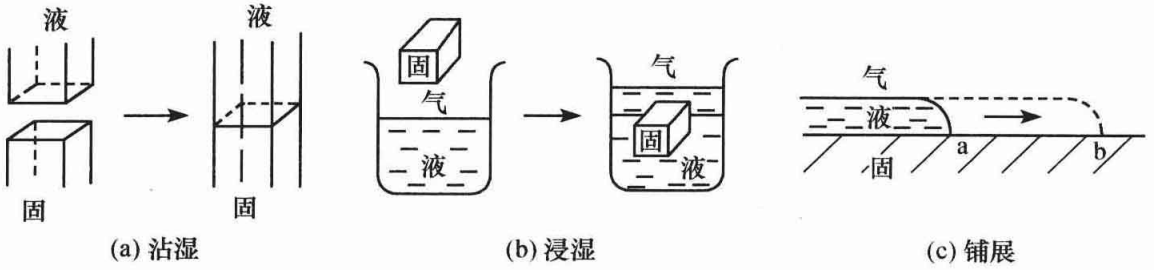
\includegraphics[width=.6\linewidth]{figures/fig8.17.png}
    \end{figure}

\end{frame}


\begin{frame}
    \frametitle{接触角与润湿作用}

    设液体在固体表面上形成液滴，达到平衡时，液滴呈现一定的形状。
    \begin{figure}[htpb]
        \centering
        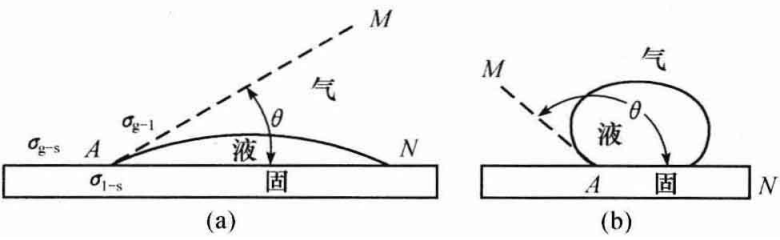
\includegraphics[width=.6\linewidth]{figures/fig8.18.png}
    \end{figure}
    $\theta$称为接触角或润湿角，大小与三种界面张力的相对大小有关，可用实验测定。

    在A点受到三种界面张力的相互作用，气-固界面张力力图使液滴沿固体表面$NA$铺开，遮盖固体表面；气-液界面张力和液-固界面张力则力图使液滴收缩，当达到平衡时，A点受合力为零，因此有
    \[
        \sigma_{\mathrm{g-s}} = \sigma_{\mathrm{l-s}} + \sigma_{\mathrm{g-l}} \cos \theta
    \]

\end{frame}


\begin{frame}
    \frametitle{接触角与润湿作用}
    \[
        \cos \theta = \frac{\sigma_{\mathrm{g-s}} - \sigma_{\mathrm{l-s}}}{\sigma_{\mathrm{g-l}}}
    \]
    上式称为杨氏（Young）方程，它是描述润湿过程的基本方程。
    \begin{itemize}
        \item 如果$\sigma_{\mathrm{g-s}} - \sigma_{\mathrm{l-s}} = \sigma_{\mathrm{g-l}}$，则$\cos \theta=1$，$\theta = 0$，这是完全润湿的情况
        \item 如果$\sigma_{\mathrm{g-s}} - \sigma_{\mathrm{l-s}} < \sigma_{\mathrm{g-l}}$，则$0<\cos \theta<1$，$\theta < 90^{\circ}$，这时固体能被液体润湿
        \item 如果$\sigma_{\mathrm{g-s}} - \sigma_{\mathrm{l-s}} > \sigma_{\mathrm{g-l}}$，则$\cos \theta<0$，$\theta > 90^{\circ}$，这时固体不能被液体润湿
    \end{itemize}
    \[
        \begin{cases}
            W_\mathrm{a} = - \sigma_{\mathrm{g-l}} (1 + \cos \theta) \\
            W_\mathrm{i} = - \sigma_{\mathrm{g-l}} (\cos \theta) \\
            S = \sigma_{\mathrm{g-l}}(1 - \cos \theta)
        \end{cases}
    \]

\end{frame}


\begin{frame}[t]
    \frametitle{}

    \begin{example}
        已知水-石墨体系的下述数据：在298K时，水的表面张力$\sigma_{\mathrm{g-l}} = \SI{0.072}{N.m^{-1}}$，测得水与石墨的接触角为90°。求水与石墨的黏附功、浸湿功和铺展系数。
    \end{example}

\end{frame}


\begin{frame}[t]
    \frametitle{}

    \begin{example}
        293K时，水的表面张力为$\SI{0.072}{N.m^{-1}}$，汞的表面张力为$\SI{0.483}{N.m^{-1}}$，而汞和水的界面张力为$\SI{0.373}{N.m^{-1}}$，试判断（1）水能否在汞的表面上铺展开；（2）汞能否在水的表面上铺展开。
    \end{example}

\end{frame}
\end{document}